\chapter{Introduction}
\label{chap:introduction}

\section{Image Compression}

Image compression is to decrease the size of the image file without dramatically downgarding the quality of the image.

In this courework, I set out to implement a simulation of the JPEG (Joint Photographic Experts Group) image compression process\citep{wallace1992jpeg}. The implementation uses MATLAB as frontend interface and Python as backend.

\section{JPEG Standard}

The JPEG Still Picture Compression Standard is widely used on modern digital devices, ranging from computers, cameras to smartphones. For a grayscale image, a JPEG CODEC (Encoder and Decoder) typically involves 6 main steps as illustrated in Figure \ref{fig:codec}.

\begin{figure}
\centering
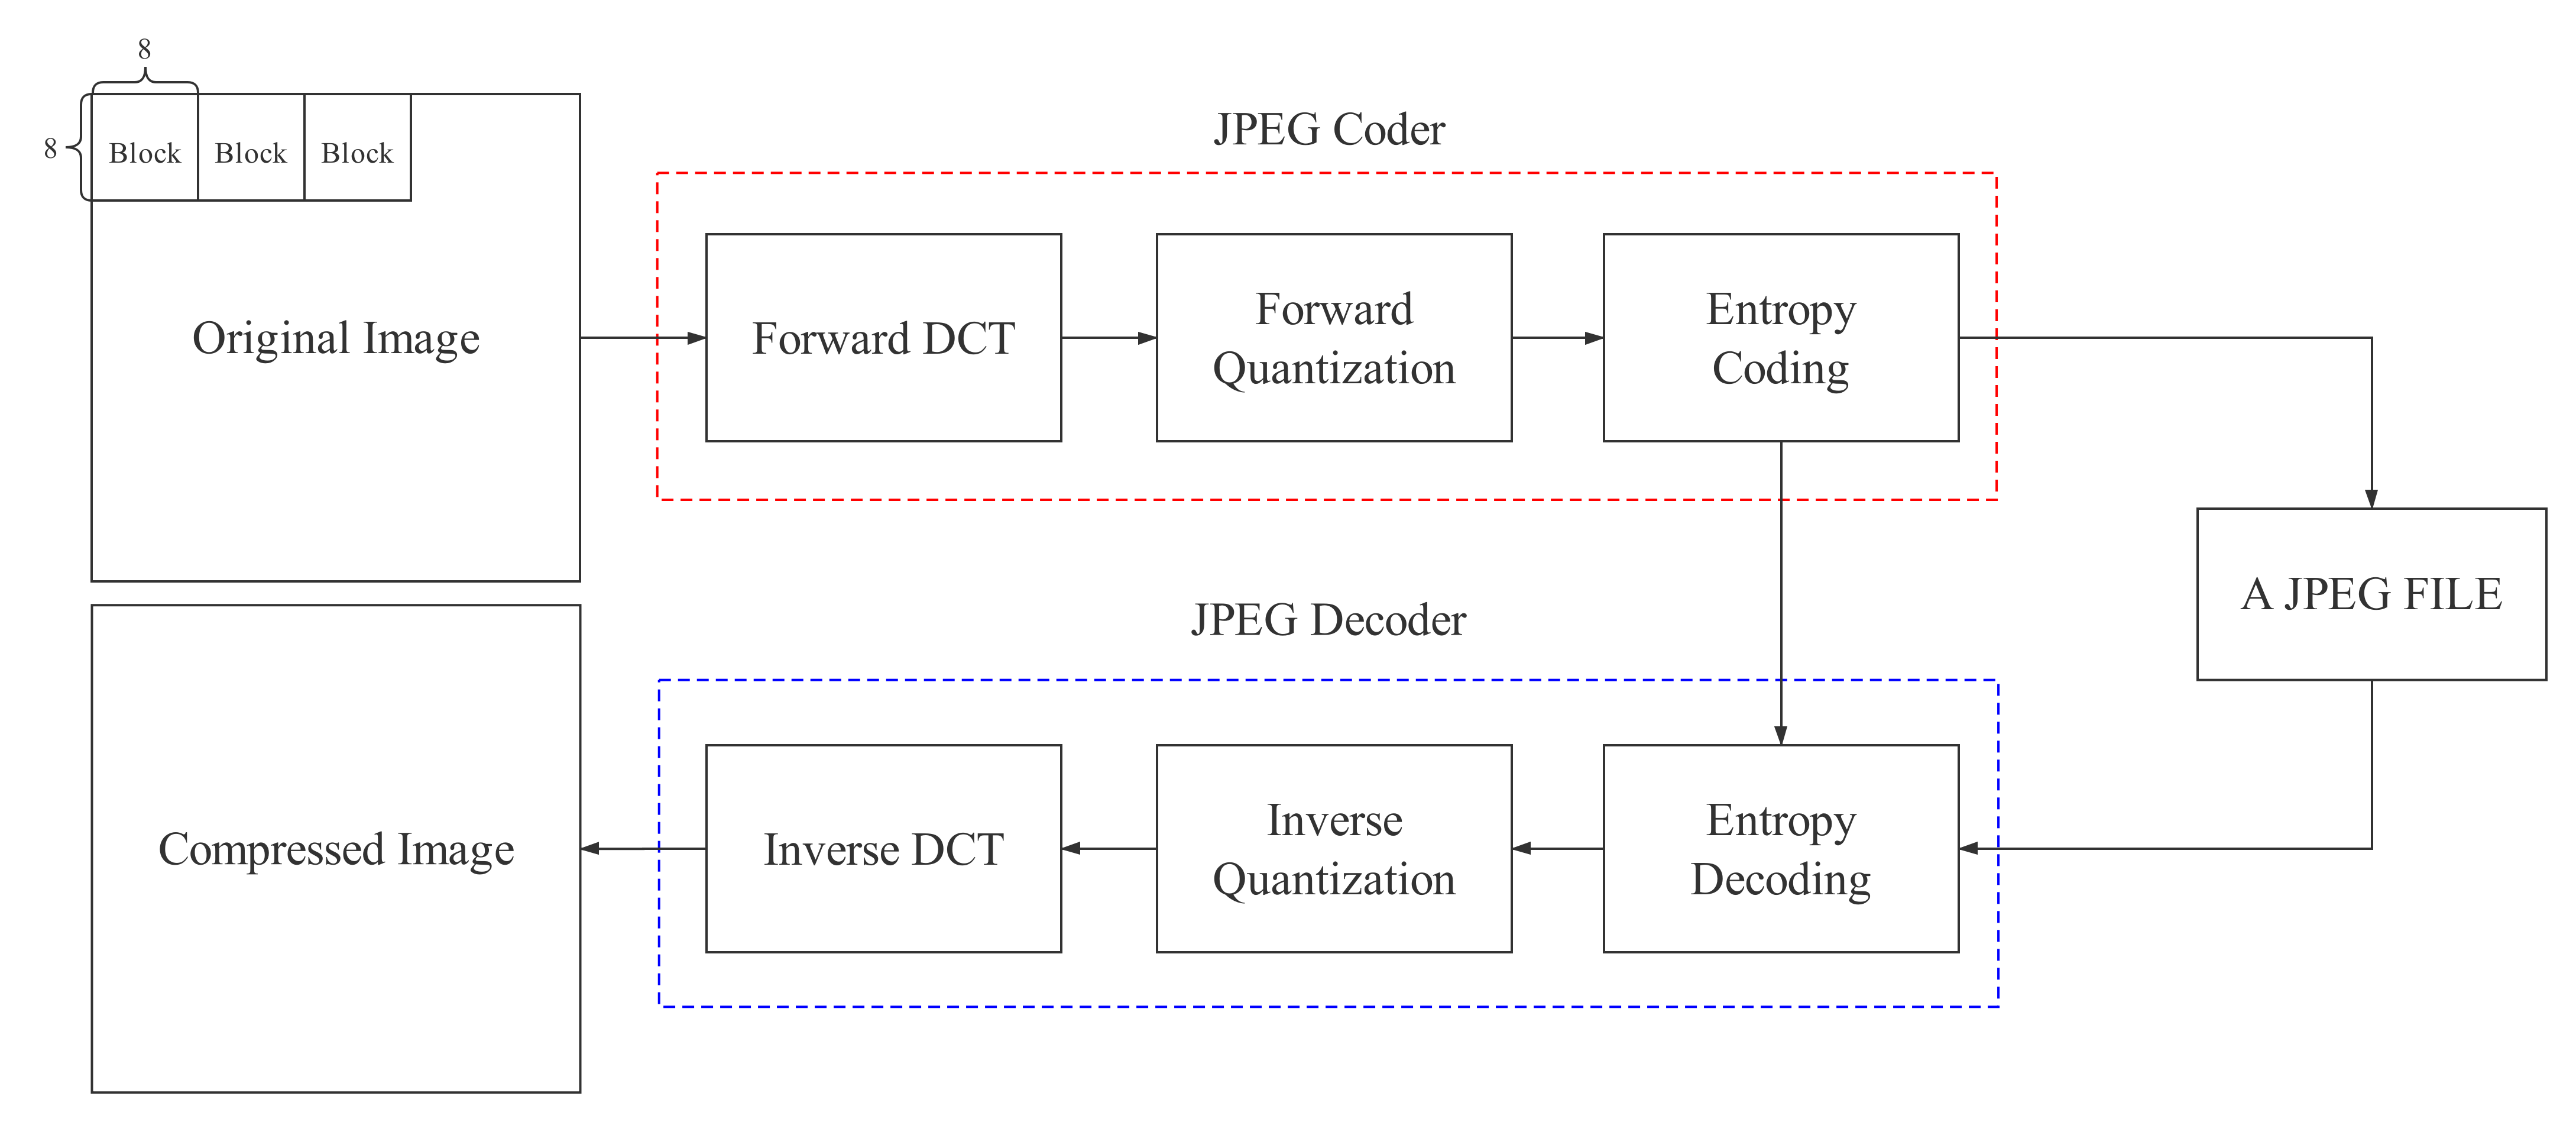
\includegraphics{codec}
\caption{Six Main Steps of a JPEG CODEC.}
\label{fig:codec}
\end{figure}

In my application, I implement a simplified JPEG CODEC in Python programming language. The CODEC consists of both foward and inverse steps of Discrete Cosine Transform (DCT) and Quantization and gets rid of both forward and inverse steps of Entropy Coding. 

Since Entropy Codeing is reversible through Inverse Entropy Coding and does not affect the quality of the image, my implementation should be able to simulate the full effects of JPEG coding on any given still image despite its simplicity.

As shown in Figure \ref{fig:app}, given an input grayscale image in uint8 matrix format, the application first crops the image array to multiply of $8$ in both column (width) and row (height). Then, a value of $128$ is subtracted from the image for each pixel value. After that, the matrix is divided into 8 by 8 blocks. Each block then goes through FDCT, Quantization, Inverse Quantization and IDCT individually.  All resulted blocks are placed in their previous position and a new matrix is thus formed. Finally, a value of $128$ is added back to the new matrix to get the compressed grayscale image. 

\begin{figure}
\centering
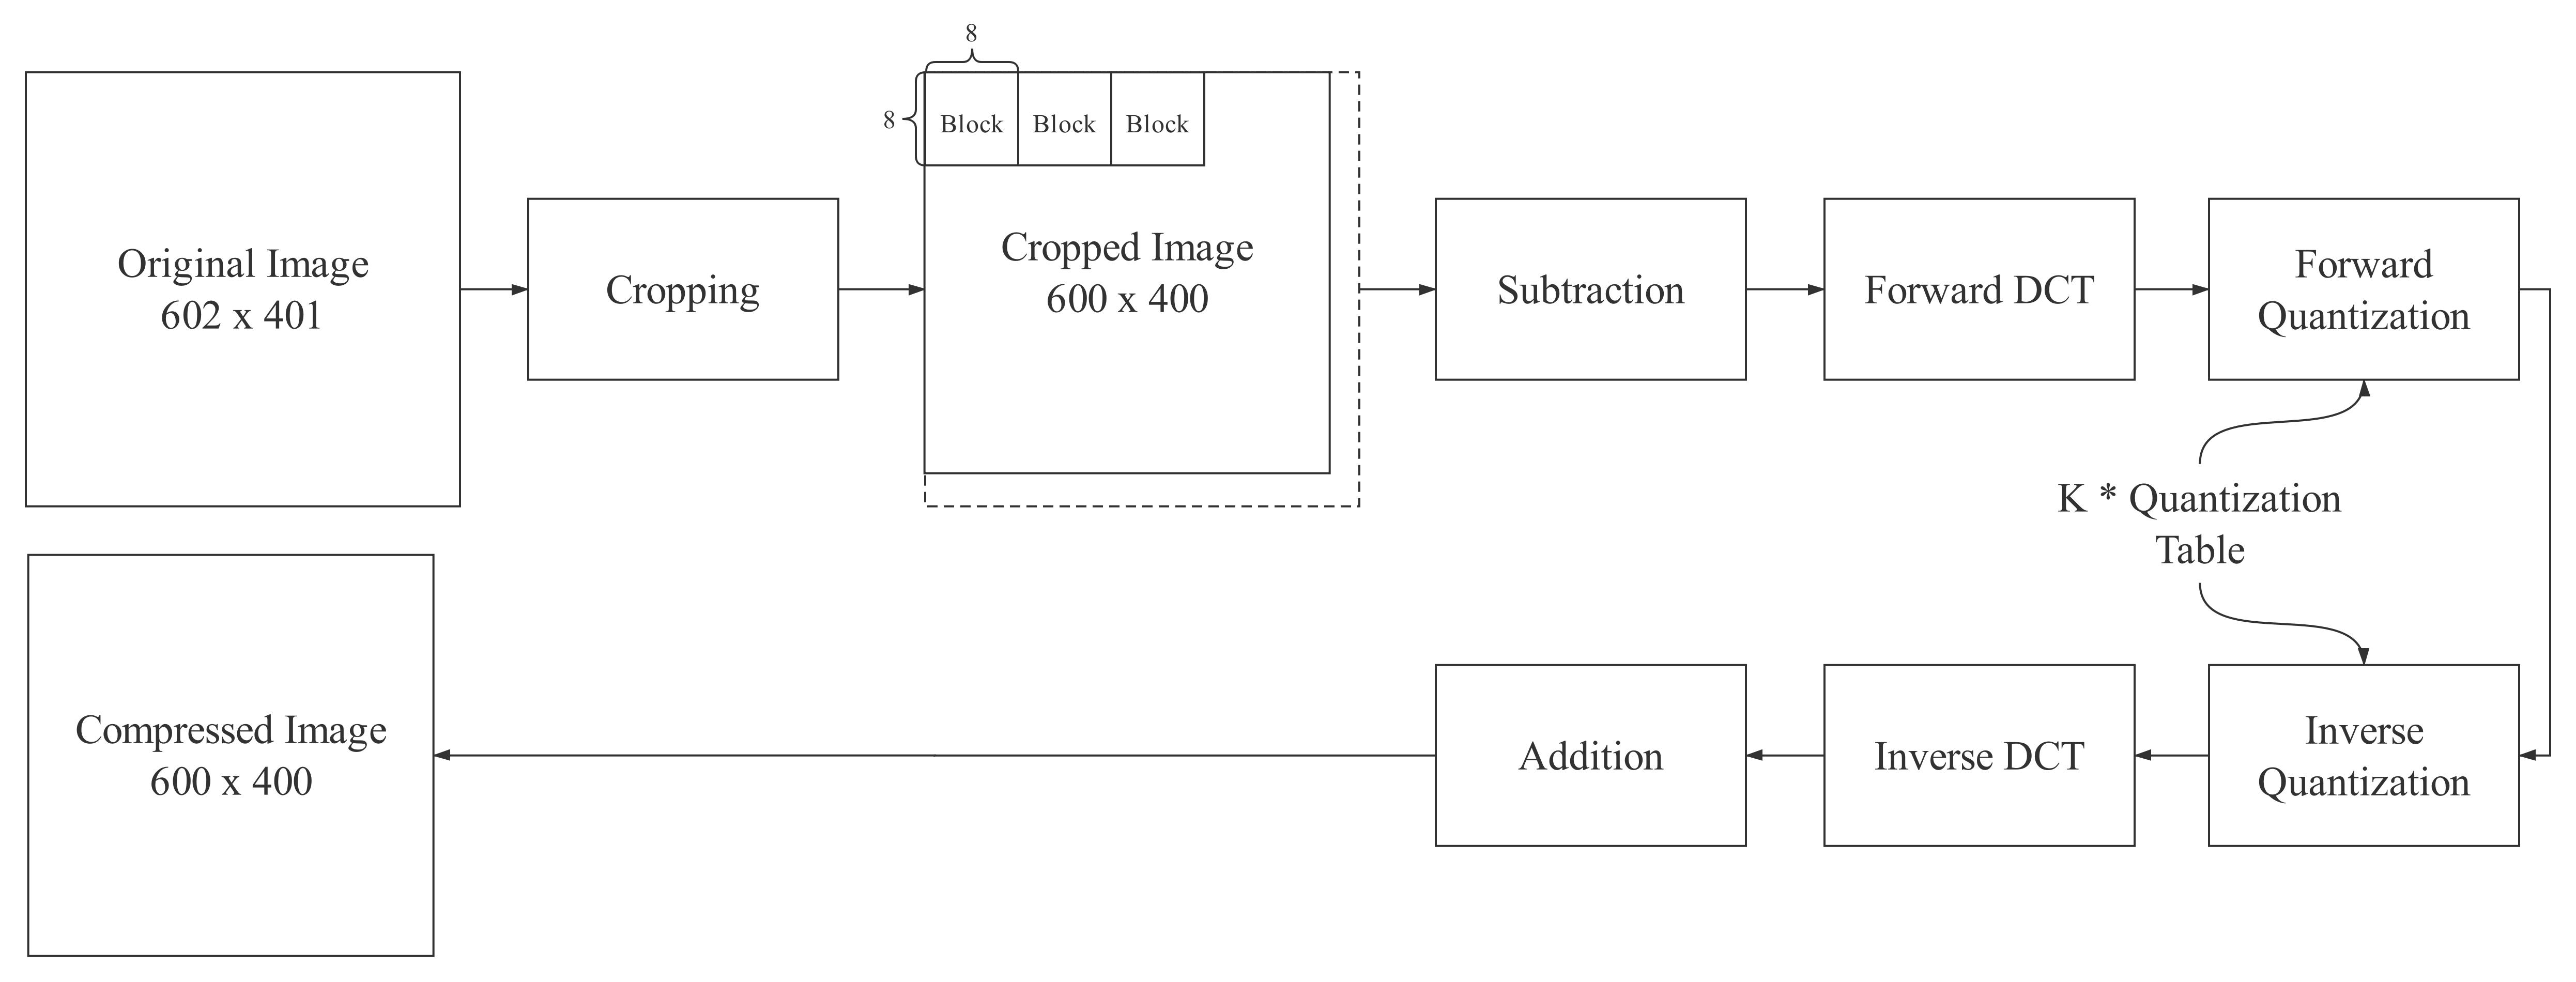
\includegraphics{app}
\caption{Main Steps of the Application.}
\label{fig:app}
\end{figure}

For a color RGB image, the same process is carried out on each color channel respectively.

\subsection{Discrete Cosine Transform (DCT)}

The forward step of DCT is computed using the following equation.

\begin{equation}
F(u, v) = \frac{1}{4} C(u) C(v) [\sum_{x=0}^7 \sum_{y=0}^7 f(x,y) * cos\frac{(2x+1)u\pi}{16} cos\frac{(2y+1)v\pi}{16}]
\label{equ:fdct}
\end{equation}

where $C(t) = 1/\sqrt(2)$ for $t = 0$; $C(t) = 1$ otherwise. Both input $f$ and output $F$ is an 8 by 8 block.

The inverse step of DCT is computed using the following equation.

\begin{equation}
f(x, y) = \frac{1}{4} [\sum_{u=0}^7 \sum_{v=0}^7 C(u) C(v) F(u, v) * cos\frac{(2x+1)u\pi}{16} cos\frac{(2y+1)v\pi}{16}]
\label{equ:idct}
\end{equation}

where $C(t) = 1/\sqrt(2)$ for $t = 0$; $C(t) = 1$ otherwise. Both input $F$ and output $f$ is an 8 by 8 block.

\subsection{Quantization}

The forward step of Quantization is computed using the following equation.

\begin{equation}
F^Q(u, v) = round(\frac{F(u, v)}{Q(u, v)})
\label{equ:fq}
\end{equation}

where $Q$ is the Quantization Table specified in the JPEG standard. Both input $F$ and ouput $F^Q$ is an 8 by 8 block.

The inverse step of Quantization is computed using the following equation.

\begin{equation}
F(u, v) = F^Q(u, v) * Q(u, v))
\label{equ:iq}
\end{equation}

where $Q$ should be the same as in the forward step. Both input $F^Q$ and ouput $F$ is an 8 by 8 block.

By default, the value of $Q$ is specfied as followed.

\begin{equation}
Q = 
\begin{bmatrix}
  16& 11& 10& 16& 24& 40& 51& 61 \\
  12& 12& 14& 19& 26& 58& 60& 55 \\
  14& 13& 16& 24& 40& 57& 69& 56 \\
  14& 17& 22& 29& 51& 87& 80& 62 \\
  18& 22& 37& 56& 68& 109& 103& 77 \\
  24& 35& 55& 64& 81& 104& 113& 92 \\
  49& 64& 78& 87& 103& 121& 120& 101 \\
  72& 92& 95& 98& 112& 100& 103& 99
\end{bmatrix}
\label{equ:q}
\end{equation}







